\section{数据库设计}
\subsection{ER图}
实体为矩形,属性为椭圆,关系为菱形。联系用线连接实体和关系,表示实体间的联系。关系有一对一、一对多、多对多三种情况。
\begin{figure}[H]
\centering
\includegraphics[width=0.8\textwidth]{image/ER图.jpg}
\caption{ER图}
\end{figure}
\subsubsection{例题}
\begin{figure}[H]
\centering
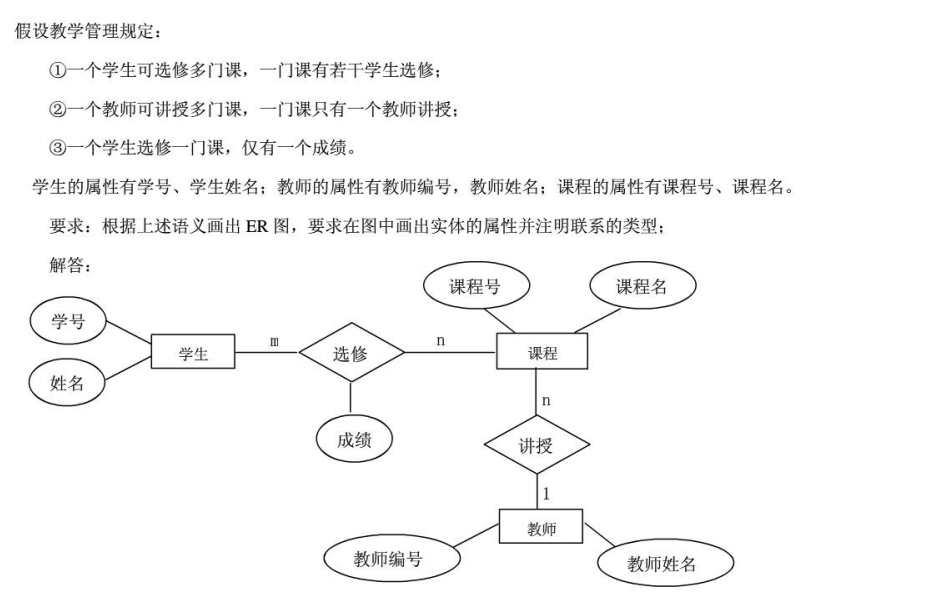
\includegraphics[width=0.8\textwidth]{image/ER图例题.png}
\caption{ER图例题}
\end{figure}

